\documentclass[t]{beamer}
\usepackage{graphicx}
\usepackage{amsmath,amsfonts,amssymb}
%exclude navigation symbols
\beamertemplatenavigationsymbolsempty
%\usetheme[compress]{default}
\usecolortheme{seagull}
\usefonttheme{structurebold}
\expandafter\def\expandafter\insertshorttitle\expandafter{\insertshorttitle\hfill\insertframenumber\,/\,\inserttotalframenumber}
\title[The RNA Workbench]{The RNA Workbench - reproducible, transparent, and accessible RNA research}
\author[RNA Workbench Team]{Florian Eggenhofer, Bj\"orn Gr\"uning, B\'{e}r\'{e}nice Batut, J\"org Fallmann, Andrea Bagnacani, Peter F. Stadler, Rolf Backofen and the RNA Workbench Team}
\institute[Bioinf]{Lehrstuhl Bioinformatik\\University of Freiburg}
\date{30.06.2017}
\subject{}
\keywords{}

\newcommand{\backupbegin}{
   \newcounter{finalframe}
   \setcounter{finalframe}{\value{framenumber}}
}
\newcommand{\backupend}{
   \setcounter{framenumber}{\value{finalframe}}
}

%\newcommand{\TODO}[1]{{\color{red} #1}}
\defbeamertemplate{footline}{higher page number}
{%
  \hfill%
  \usebeamercolor[fg]{page number in head/foot}%
  \usebeamerfont{page number in head/foot}%
  \raisebox{0.2cm}[0pt][0pt]{
  \insertframenumber\,/\,\inserttotalframenumber\kern1em}%
}
\setbeamertemplate{footline}[higher page number]
\begin{document}
\frame{
  \titlepage
}

%% \frame{
%%   \frametitle{Goals of the RNA Workbench}
%%   %Differences to previous work
%%   %\onslide<1->
%%   \begin{figure}
%%     \only<1>{
\includegraphics[width=0.5\textwidth]{figures/welcome_image_1.eps}}
%%     \only<2>{\hspace{-3.5pt}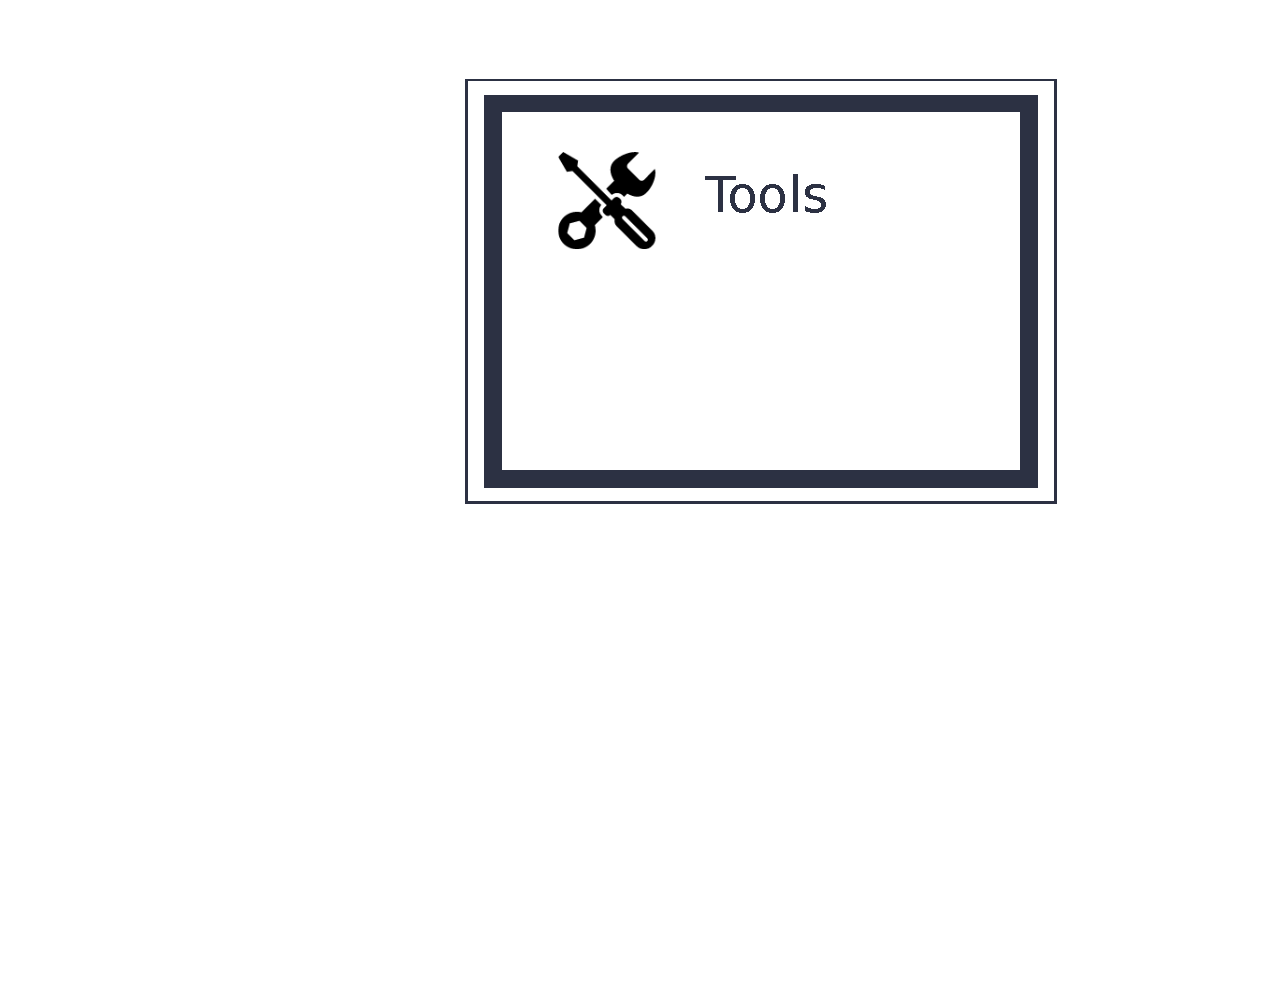
\includegraphics[width=0.5\textwidth]{figures/welcome_image_2.eps}}
%%     \only<3>{\hspace{-7pt}
\includegraphics[width=0.5\textwidth]{figures/welcome_image_3.eps}}
%%     \only<4>{\hspace{-10.5pt}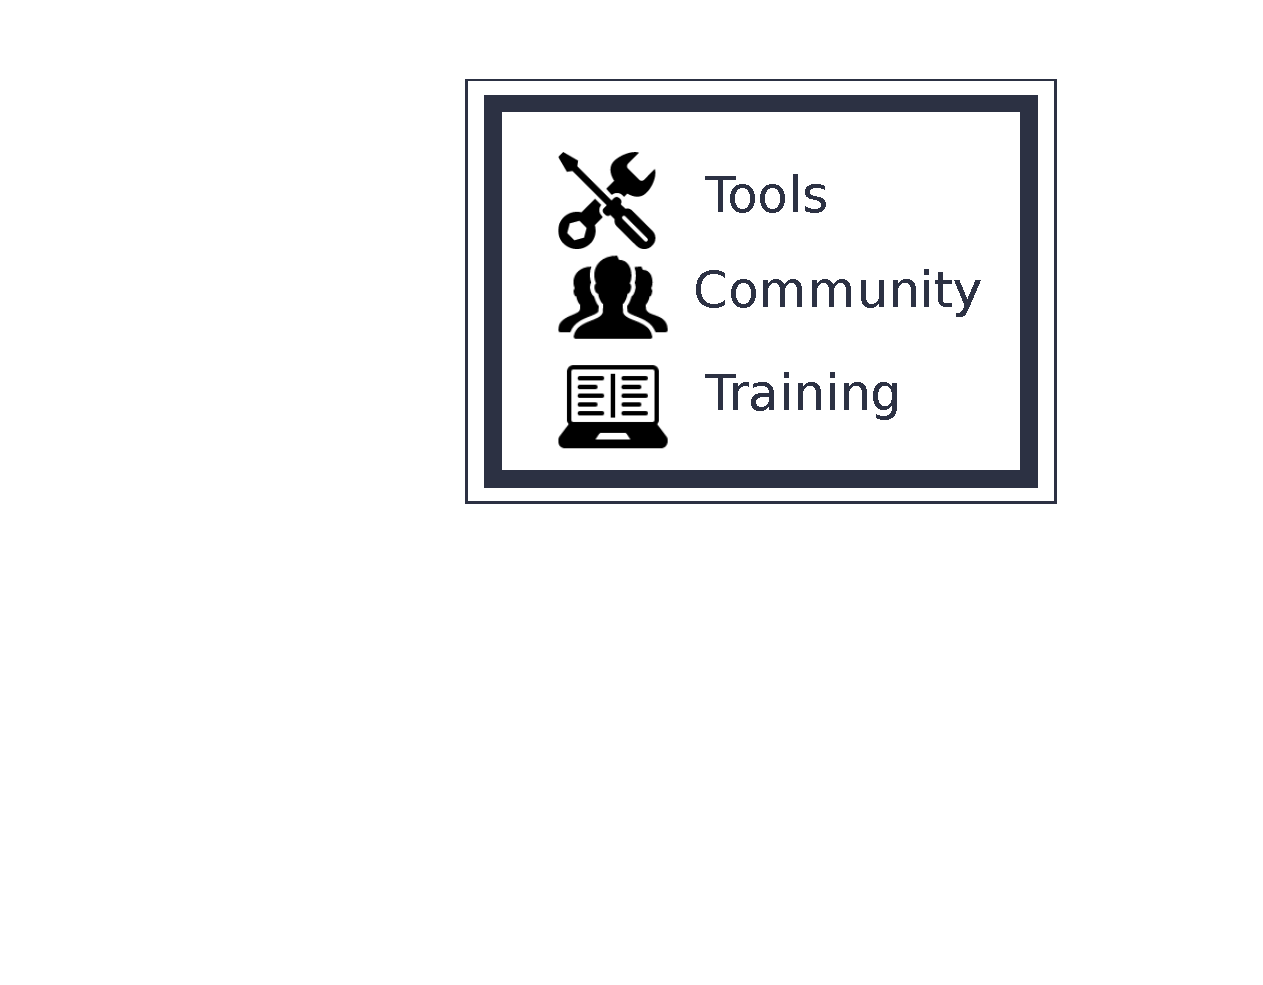
\includegraphics[width=0.5\textwidth]{figures/welcome_image_4.eps}}
%%     \only<5>{\hspace{-14pt}
\includegraphics[width=0.5\textwidth]{figures/welcome_image_5.eps}}
%%     \only<6>{\hspace{-14pt}
\includegraphics[width=0.5\textwidth]{figures/welcome_image.eps}}
%%   \end{figure}
%%   \begin{itemize}
%%   \item<2-> Comprehensive set of \textit{RNA}-bioinformatics tools
%%   \item<3-> Community - authors and users
%%   \item<4-> Set of predefined workflows and associated descriptions/training material
%%   \item<5-> Easy and stable dissemination via Galaxy \onslide<6->{and Docker}
%%   \end{itemize}
%% }

\frame{
  \frametitle{Goals of the \textit{RNA} Workbench}
  \begin{figure}
    
\includegraphics[width=0.5\textwidth]{figures/welcome_image_1.eps}
  \end{figure}
}

\frame{
  \frametitle{Goals of the \textit{RNA} Workbench}
  \begin{figure}
    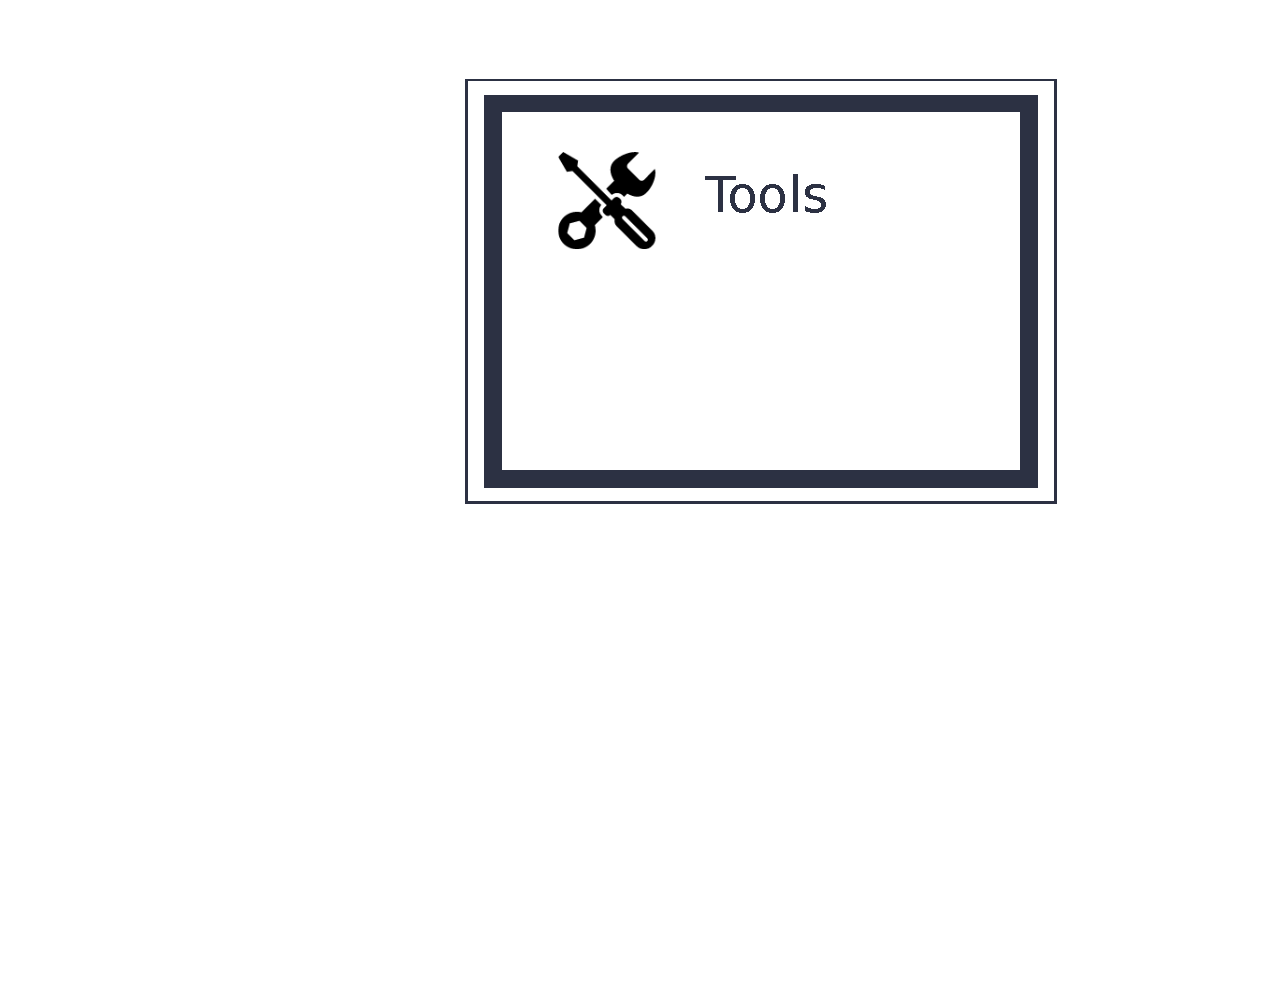
\includegraphics[width=0.5\textwidth]{figures/welcome_image_2.eps}
  \end{figure}
  \begin{itemize}
  \item Comprehensive set of \textit{RNA}-bioinformatics tools
  \end{itemize}
}

\frame{
  \frametitle{Goals of the \textit{RNA} Workbench}
  \begin{figure}
    
\includegraphics[width=0.5\textwidth]{figures/welcome_image_3.eps}
  \end{figure}
  \begin{itemize}
  \item Comprehensive set of \textit{RNA}-bioinformatics tools
  \item Community - authors and users
  \end{itemize}
}

\frame{
  \frametitle{Goals of the \textit{RNA} Workbench}
  \begin{figure}
    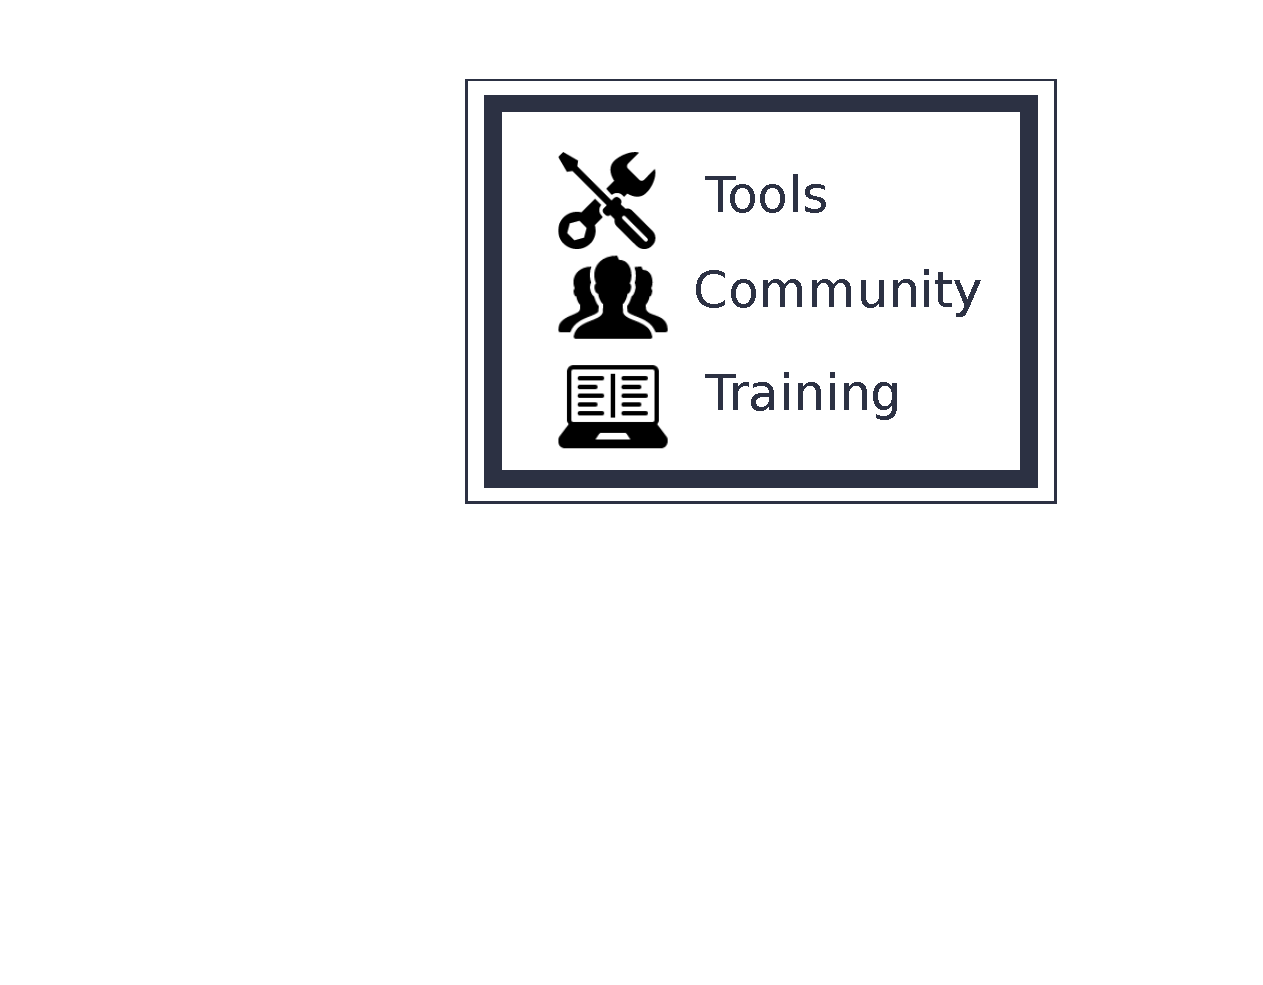
\includegraphics[width=0.5\textwidth]{figures/welcome_image_4.eps}
  \end{figure}
  \begin{itemize}
  \item Comprehensive set of \textit{RNA}-bioinformatics tools
  \item Community - authors and users
  \item Set of predefined workflows and associated descriptions/training material
  \end{itemize}
}

\frame{
  \frametitle{Goals of the \textit{RNA} Workbench}
  \begin{figure}
    
\includegraphics[width=0.5\textwidth]{figures/welcome_image.eps}
  \end{figure}
  \begin{itemize}
  \item Comprehensive set of \textit{RNA}-bioinformatics tools
  \item Community - authors and users
  \item Set of predefined workflows and associated descriptions/training material
  \item Easy and stable dissemination via Galaxy 
  \end{itemize}
}

\frame{
  \frametitle{Tools}
  %Tool logo cloud with categories
  \begin{itemize}
  \item<1-> More than \textbf{50} \textit{RNA} bioinformatics tools
  \item<2-> Classical \textit{RNA} bioinformatics (INFERNAL, ViennaRNA, ..)
  \item<3-> \textit{RNA}-seq analysis (FuMa, PARalyzer, ..)
  \item<4-> Integrated \textit{RNA} visualization
   \vspace{0.5cm}
   \begin{figure}
    \centering
    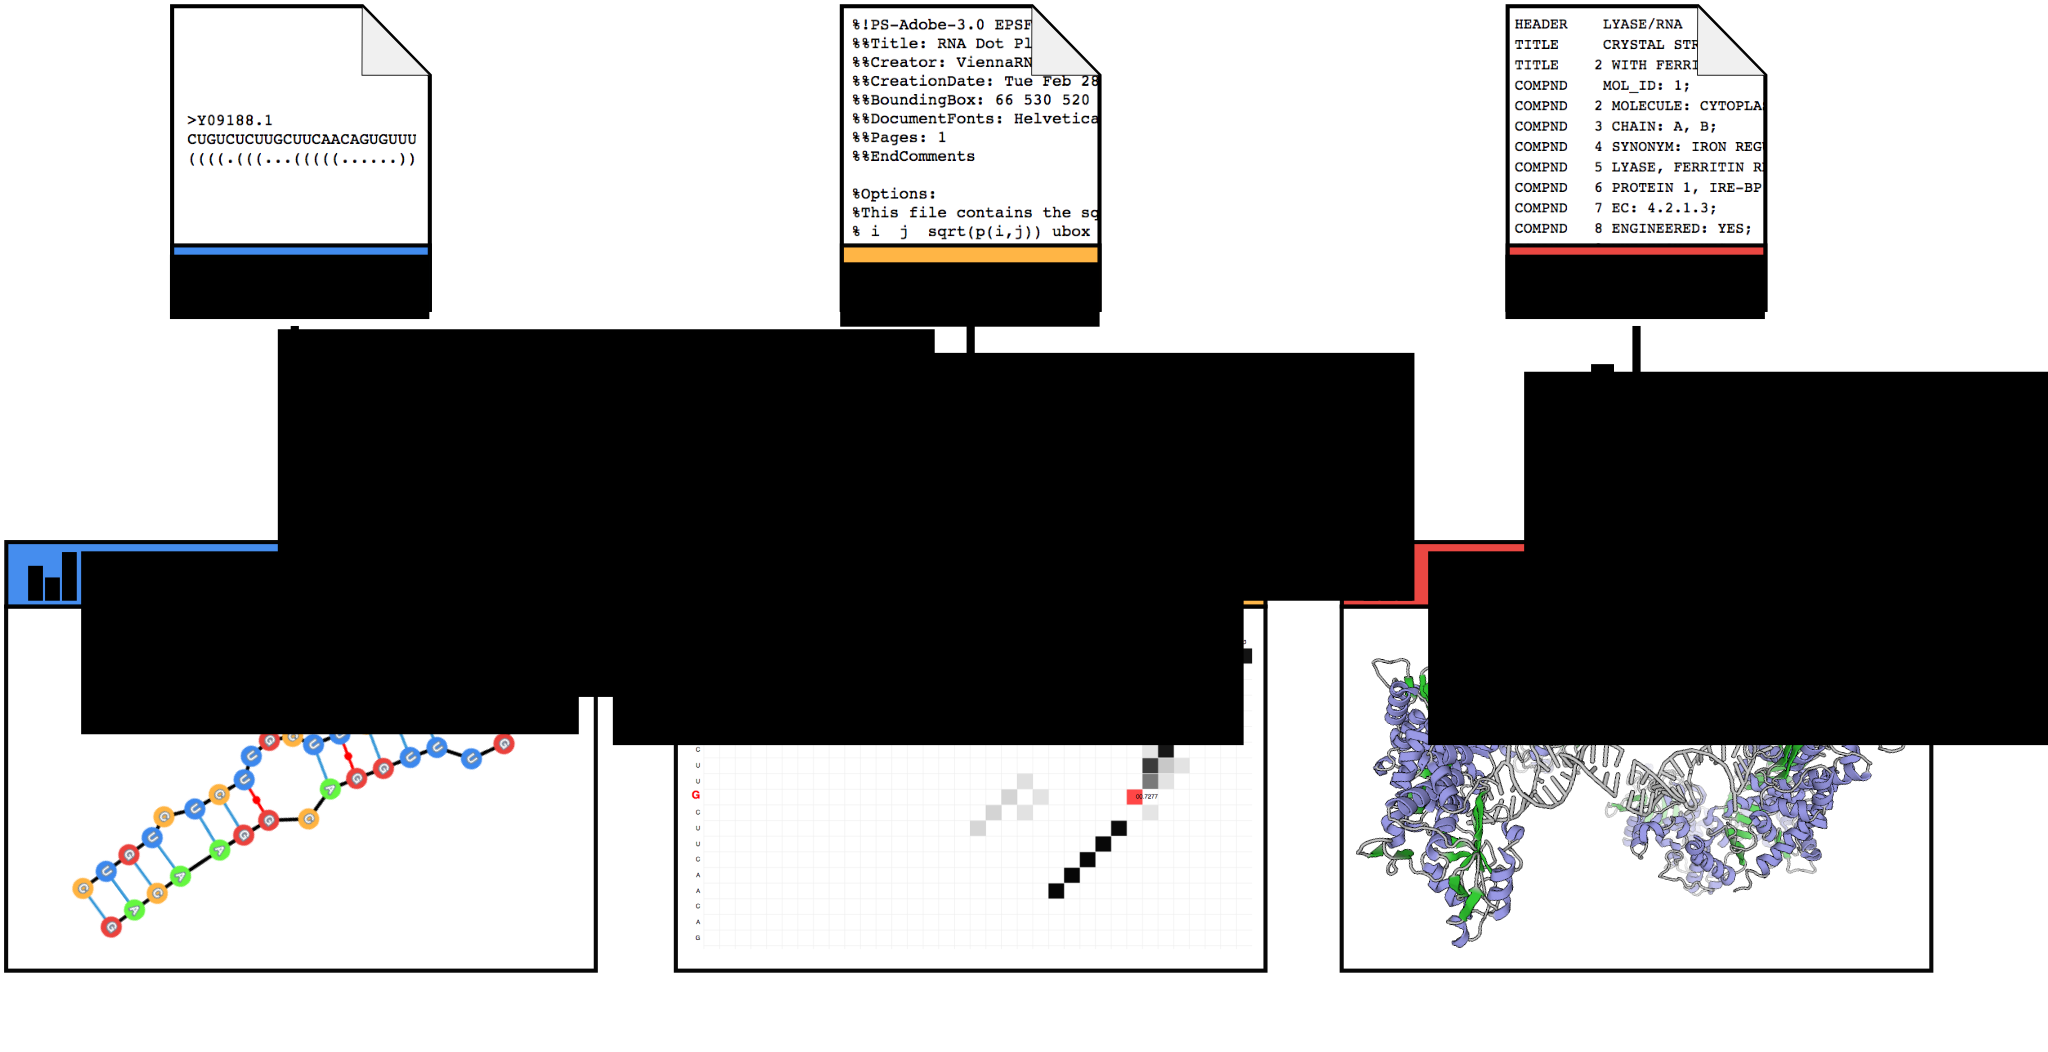
\includegraphics[width=0.7\textwidth]{figures/visualization.eps}
  \end{figure}
  \end{itemize}  
}


\frame{
  \frametitle{Workflows}
  \begin{itemize}
  \item<1-> Standardized analysis procedures
  \item<2-> Based on tools as building blocks
  \item<3-> Can be developed, adapted and shared (ToolShed/myexperiment.org)
  \begin{figure}
    \centering
    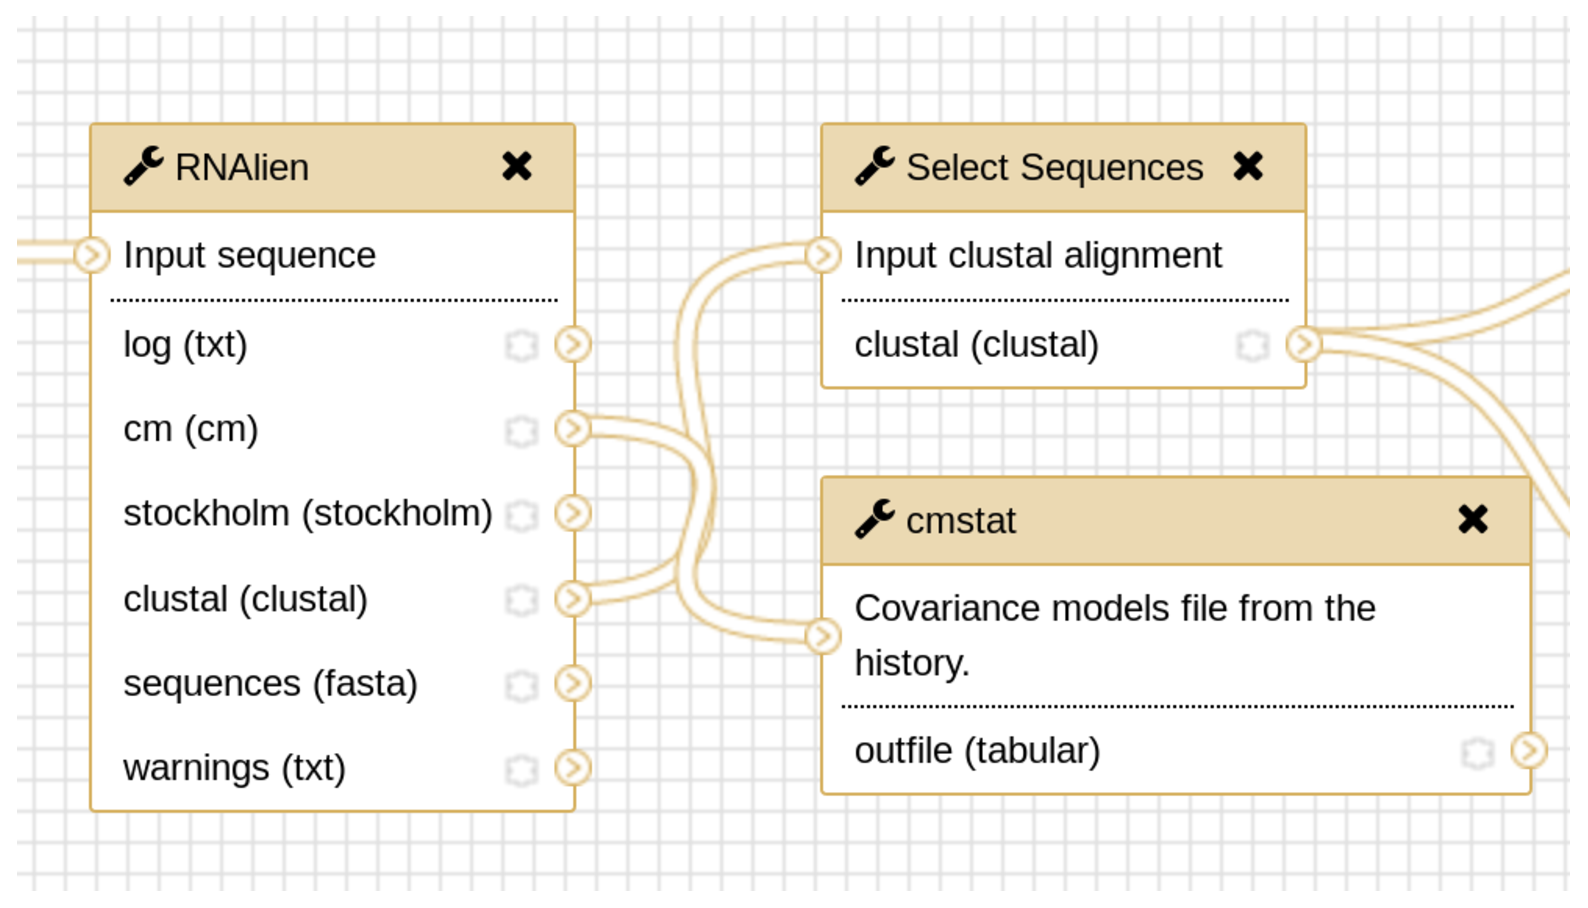
\includegraphics[width=0.5\textwidth]{figures/workflowdesign.eps}
  \end{figure}
  \item<4-> Currently six workflows %TODO - add workflows
    \begin{itemize}
    \item<5-> \textit{ncRNA} analysis
    \item<6-> \textit{RNA} model construction
    \item<7-> \textit{RNA}-seq analysis
    \item<8-> Two workflows for CLIP analysis
    \item<9-> C/D-box scan
    \end{itemize}
  \end{itemize}
    %Turning history into workflow / design from scratch
}

%% \frame{
%%   \frametitle{Workflow - Analysis of non-coding \textit{RNA}s}
%%   \begin{itemize}
%%   \item Test for functional structure via conservation
%%   \end{itemize}
%%    \begin{figure}
%%      \centering
%%     \only<1>{
\includegraphics[width=0.8\textwidth]{figures/ncRNA_general_Workflow_1.eps}} 
%%     \only<2>{
\includegraphics[width=0.8\textwidth]{figures/ncRNA_general_Workflow_2.eps}}
%%     \only<3>{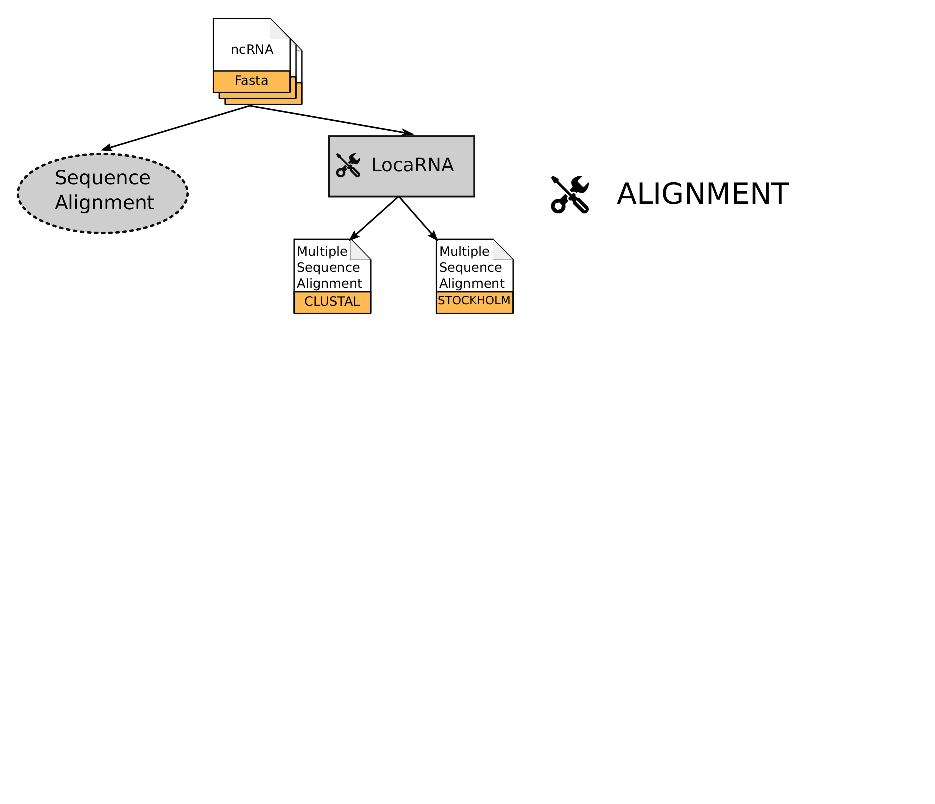
\includegraphics[width=0.8\textwidth]{figures/ncRNA_general_Workflow_3.eps}}
%%     \only<4>{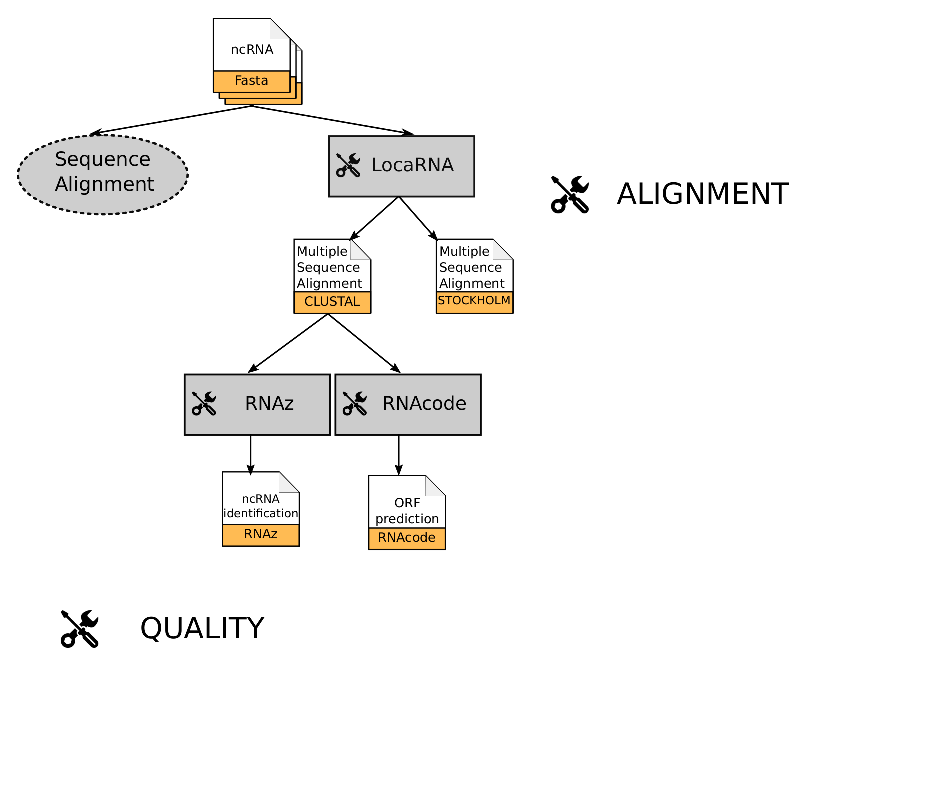
\includegraphics[width=0.8\textwidth]{figures/ncRNA_general_Workflow_4.eps}}
%%     \only<5>{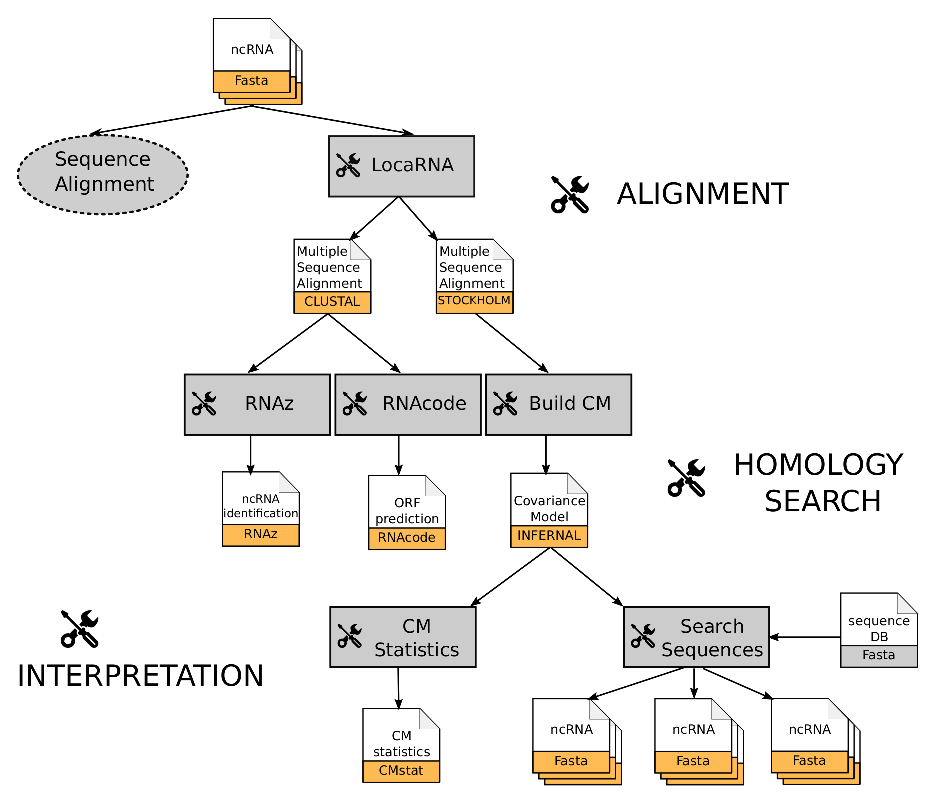
\includegraphics[width=0.8\textwidth]{figures/ncRNA_general_Workflow_5.eps}}
%%     \only<6>{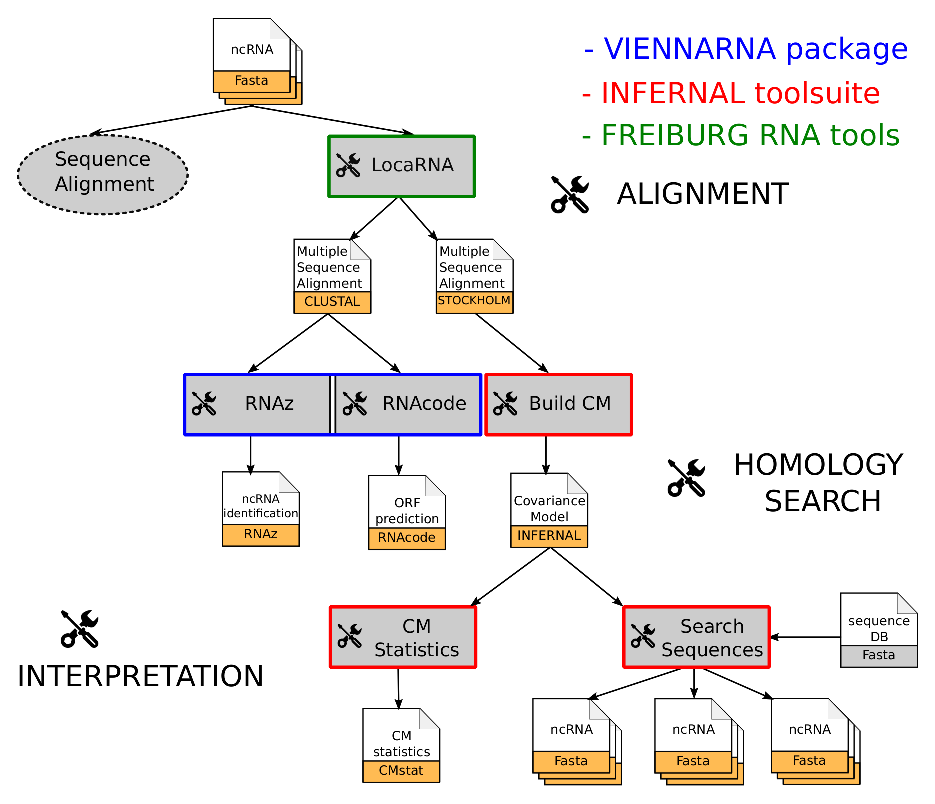
\includegraphics[width=0.8\textwidth]{figures/ncRNA_general_Workflow_6.eps}}
%%   \end{figure}
  
%% }

\frame{
  \frametitle{Workflow - Analysis of non-coding \textit{RNA}s}
  \begin{itemize}
  \item Test for functional structure via conservation
  \end{itemize}
   \begin{figure}
     \centering
     
\includegraphics[width=0.8\textwidth]{figures/ncRNA_general_Workflow_1.eps} 
  \end{figure}  
}

\frame{
  \frametitle{Workflow - Analysis of non-coding \textit{RNA}s}
  \begin{itemize}
  \item Test for functional structure via conservation
  \end{itemize}
   \begin{figure}
     \centering
     
\includegraphics[width=0.8\textwidth]{figures/ncRNA_general_Workflow_2.eps}
  \end{figure}
  
}

\frame{
  \frametitle{Workflow - Analysis of non-coding \textit{RNA}s}
  \begin{itemize}
  \item Test for functional structure via conservation
  \end{itemize}
   \begin{figure}
     \centering
     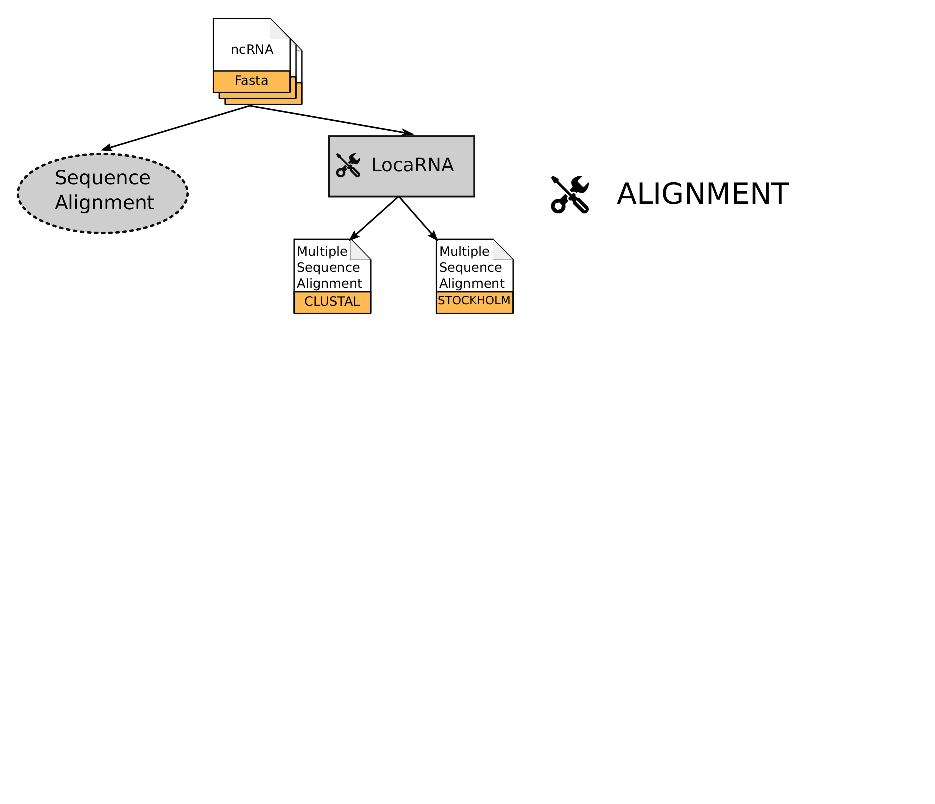
\includegraphics[width=0.8\textwidth]{figures/ncRNA_general_Workflow_3.eps}
  \end{figure}
  
}

\frame{
  \frametitle{Workflow - Analysis of non-coding \textit{RNA}s}
  \begin{itemize}
  \item Test for functional structure via conservation
  \end{itemize}
   \begin{figure}
     \centering
     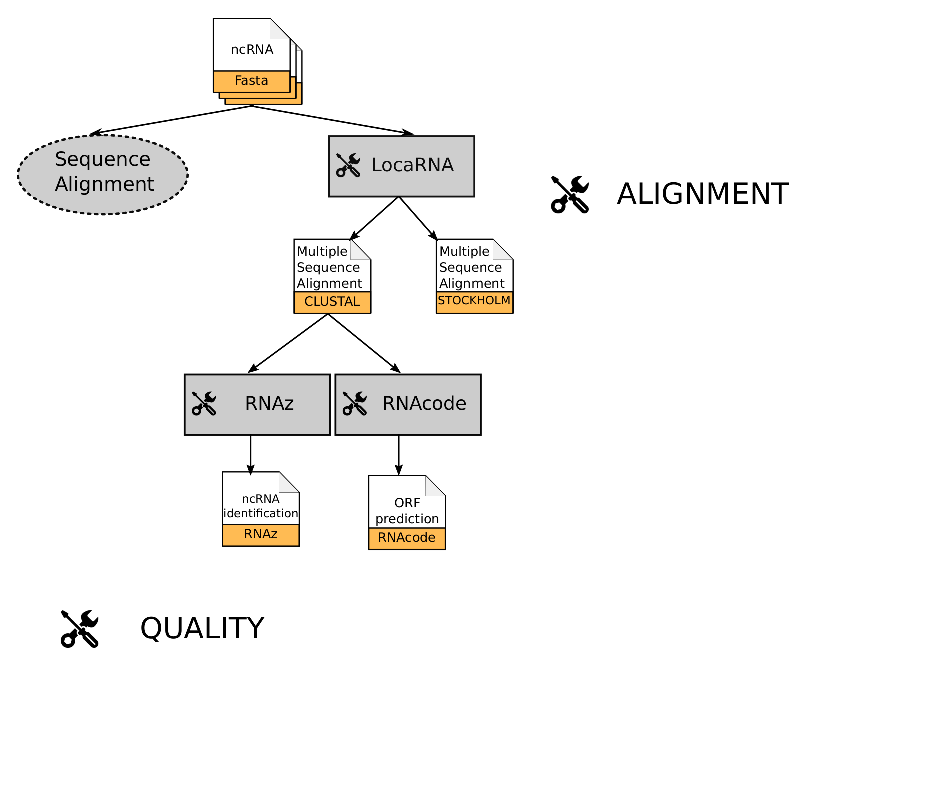
\includegraphics[width=0.8\textwidth]{figures/ncRNA_general_Workflow_4.eps}
  \end{figure}
}

\frame{
  \frametitle{Workflow - Analysis of non-coding \textit{RNA}s}
  \begin{itemize}
  \item Test for functional structure via conservation
  \end{itemize}
   \begin{figure}
     \centering
     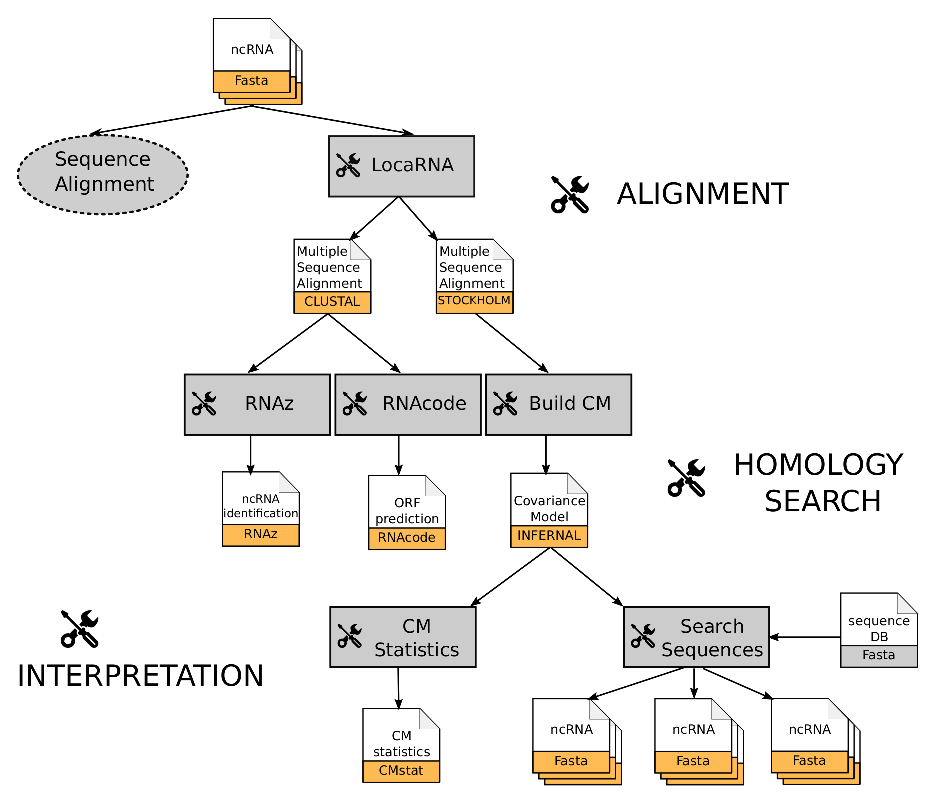
\includegraphics[width=0.8\textwidth]{figures/ncRNA_general_Workflow_5.eps}
  \end{figure}  
}

\frame{
  \frametitle{Workflow - Analysis of non-coding \textit{RNA}s}
  \begin{itemize}
  \item Test for functional structure via conservation
  \end{itemize}
   \begin{figure}
     \centering
     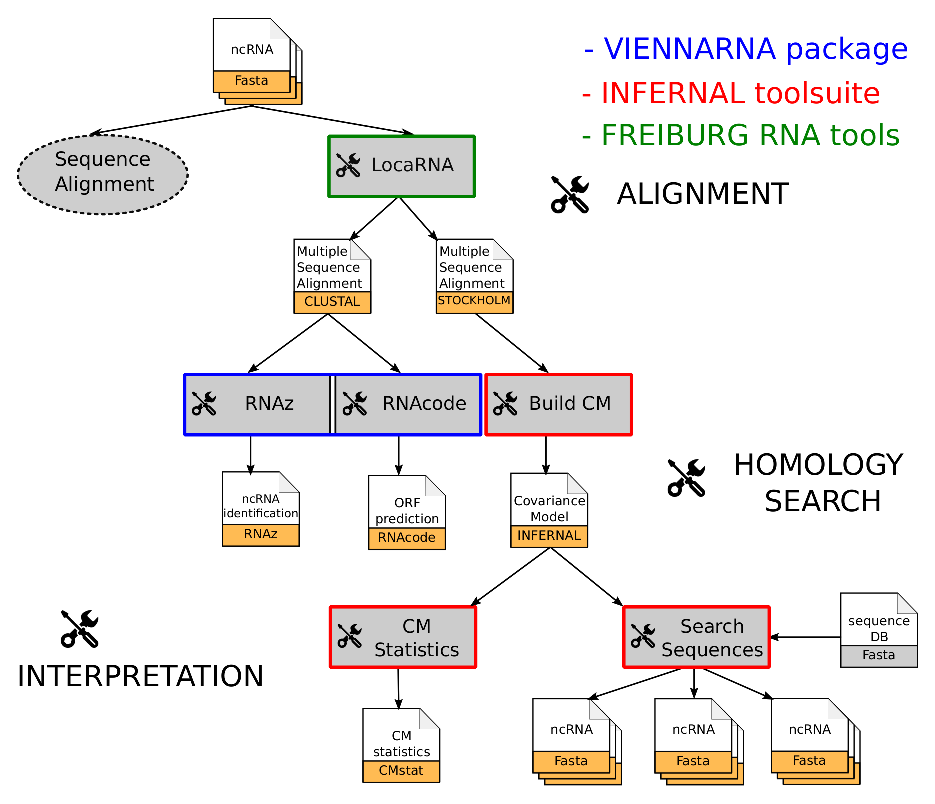
\includegraphics[width=0.8\textwidth]{figures/ncRNA_general_Workflow_6.eps}
  \end{figure}  
}

%% \frame{
%%   \frametitle{Workflow - \textit{RNA} family model construction}
%%   \begin{itemize}
%%   \item RNA family model construction
%%   \end{itemize}
%%    \begin{figure}
%%      \centering
%%     \only<1>{
\includegraphics[width=0.7\textwidth]{figures/modelconstruction_Workflow1.eps}}
%%     \only<2>{
\includegraphics[width=0.7\textwidth]{figures/modelconstruction_Workflow2.eps}}
%%     \only<3>{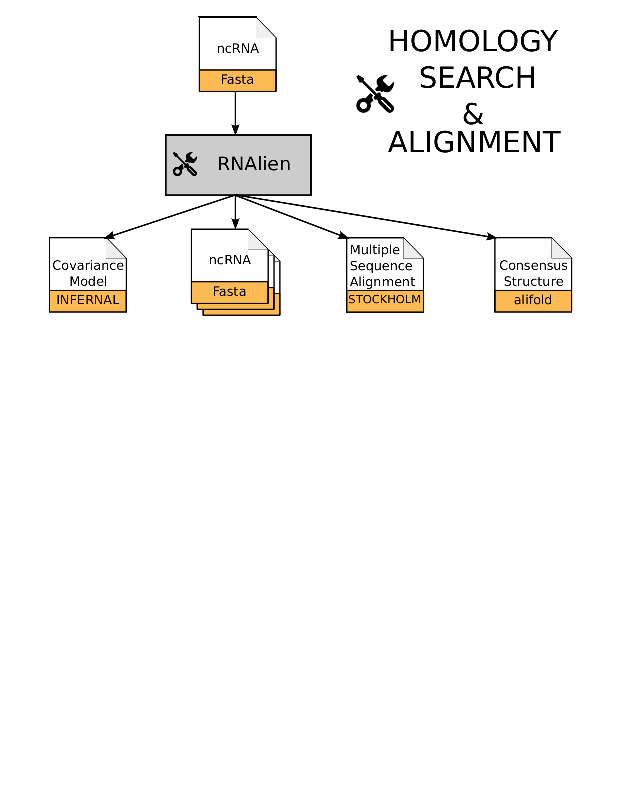
\includegraphics[width=0.7\textwidth]{figures/modelconstruction_Workflow3.eps}}
%%     \only<4>{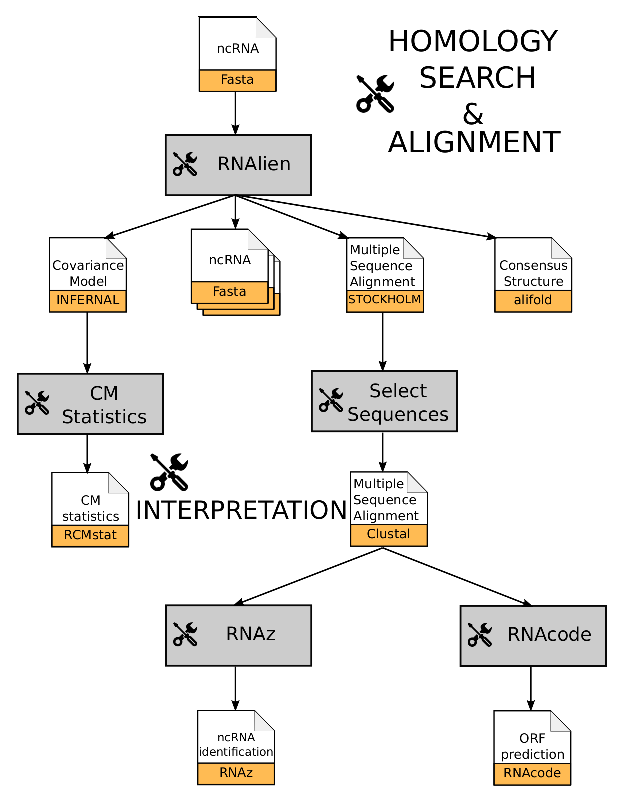
\includegraphics[width=0.7\textwidth]{figures/modelconstruction_Workflow4.eps}}
%%   \end{figure}
%% }

\frame{
  \frametitle{Workflow - \textit{RNA} family model construction}
  \begin{itemize}
  \item RNA family model construction
  \end{itemize}
   \begin{figure}
     \centering
     
\includegraphics[width=0.5\textwidth]{figures/modelconstruction_Workflow1.eps}
  \end{figure}
}

\frame{
  \frametitle{Workflow - \textit{RNA} family model construction}
  \begin{itemize}
  \item RNA family model construction
  \end{itemize}
   \begin{figure}
     \centering
     
\includegraphics[width=0.5\textwidth]{figures/modelconstruction_Workflow2.eps}
  \end{figure}
}

\frame{
  \frametitle{Workflow - \textit{RNA} family model construction}
  \begin{itemize}
  \item RNA family model construction
  \end{itemize}
   \begin{figure}
     \centering
     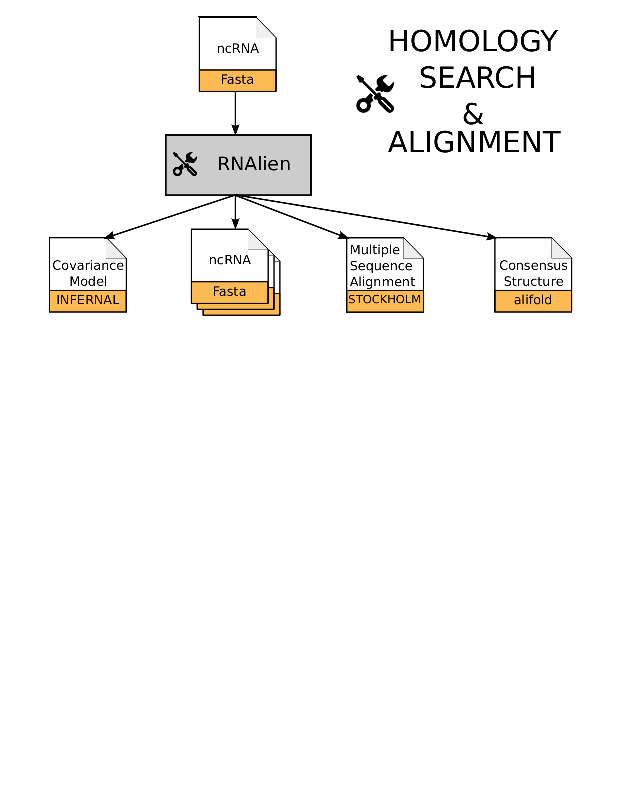
\includegraphics[width=0.5\textwidth]{figures/modelconstruction_Workflow3.eps}
  \end{figure}
}

\frame{
  \frametitle{Workflow - \textit{RNA} family model construction}
  \begin{itemize}
  \item RNA family model construction
  \end{itemize}
   \begin{figure}
     \centering
     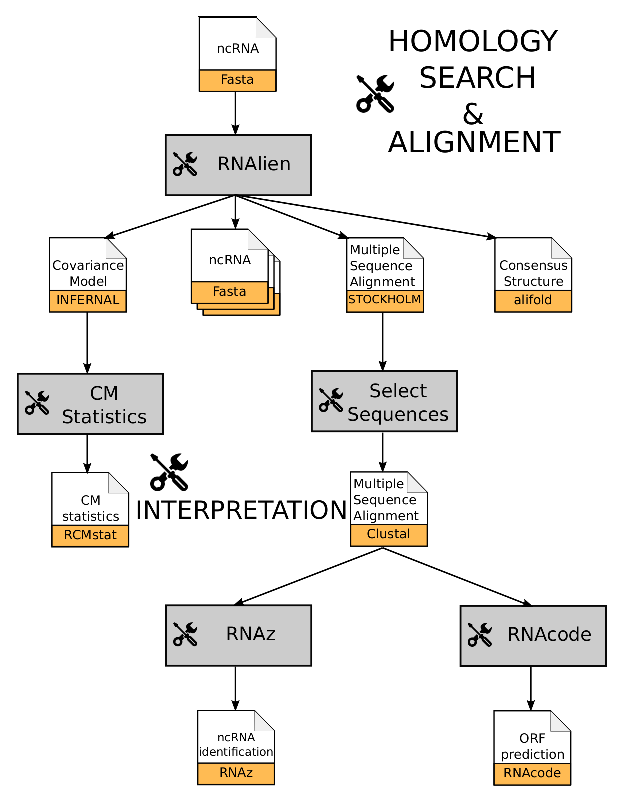
\includegraphics[width=0.5\textwidth]{figures/modelconstruction_Workflow4.eps}
  \end{figure}
}

\frame{
  \frametitle{Collaboration \& Synergistic effects}
   \begin{figure}
     \centering
     \includegraphics[width=\textwidth]{figures/ncRNAworkflows_simplified.eps}
  \end{figure}
}

\frame{
  \frametitle{Collaboration \& Synergistic effects}
   \begin{figure}
     \centering
     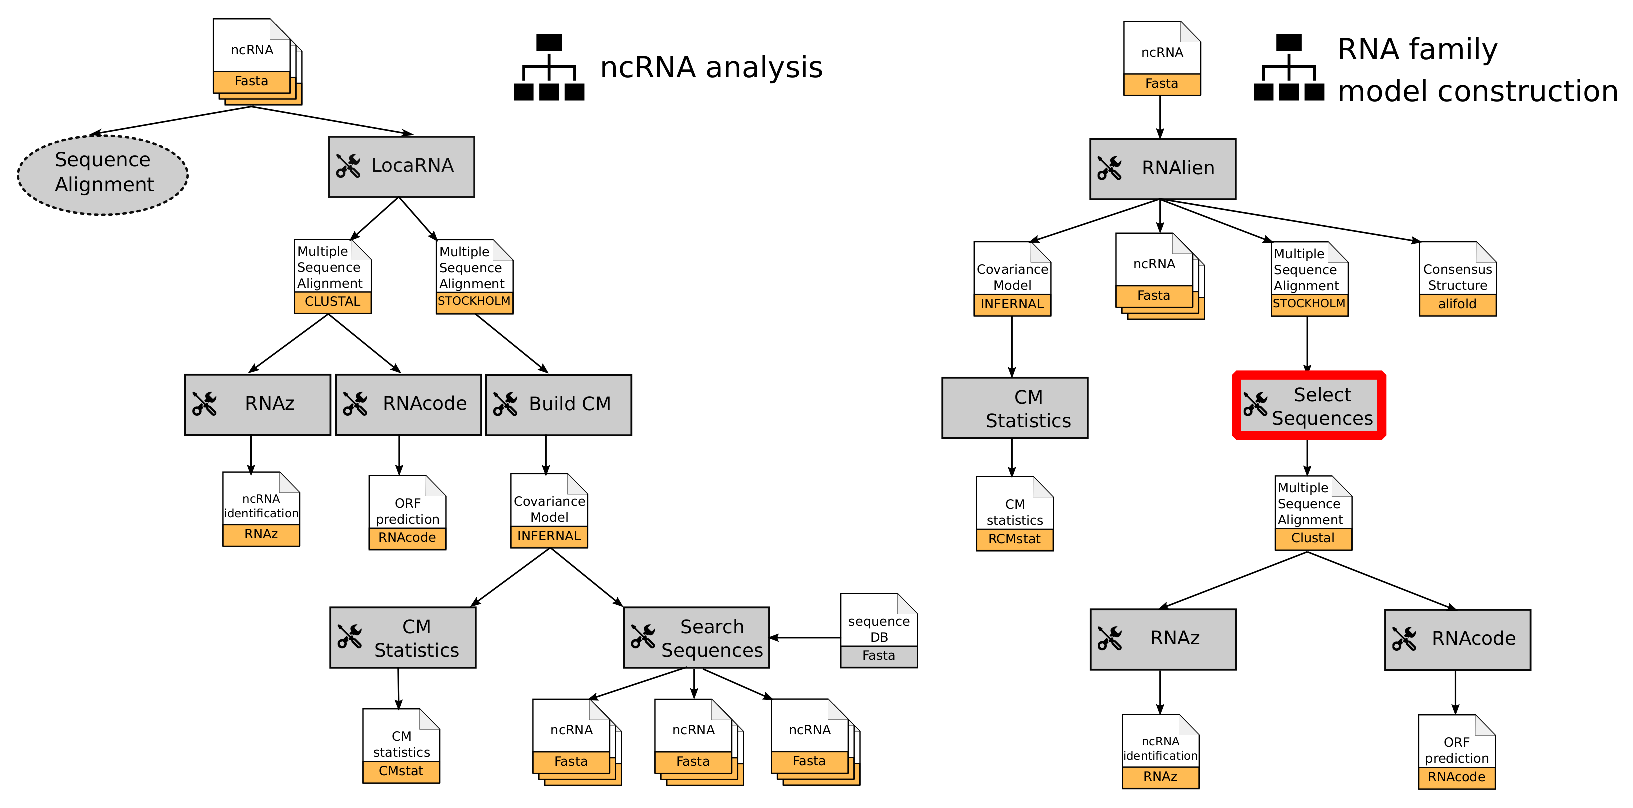
\includegraphics[width=\textwidth]{figures/ncRNAworkflows_simplified_1.eps}
  \end{figure}
}

\frame{
  \frametitle{Collaboration \& Synergistic effects}
   \begin{figure}
     \centering
     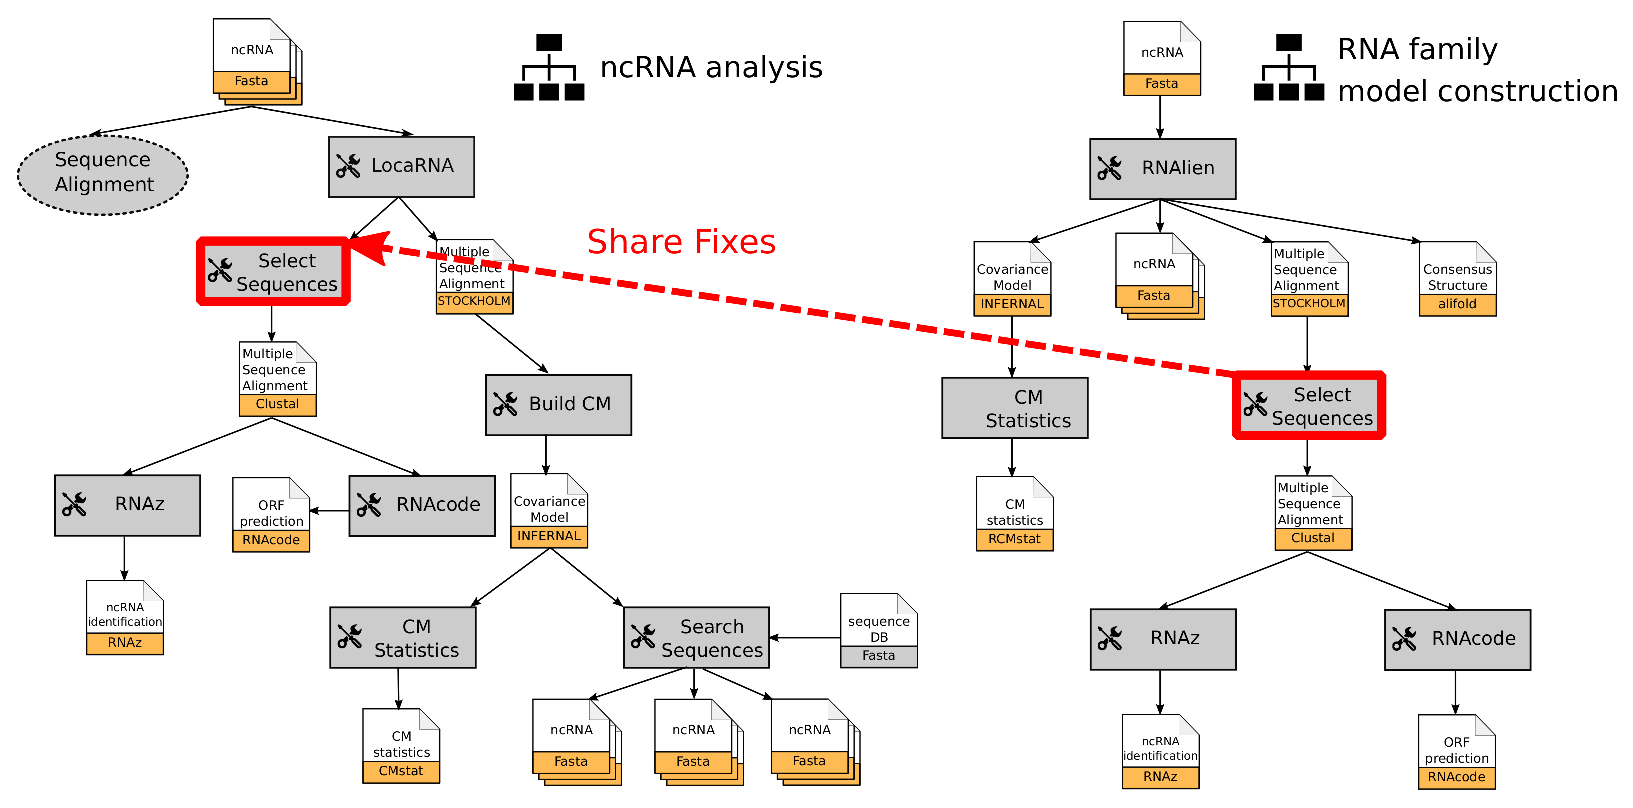
\includegraphics[width=\textwidth]{figures/ncRNAworkflows_simplified_2.eps}
  \end{figure}
}

\frame{
  \frametitle{Collaboration \& Synergistic effects}
   \begin{figure}
     \centering
     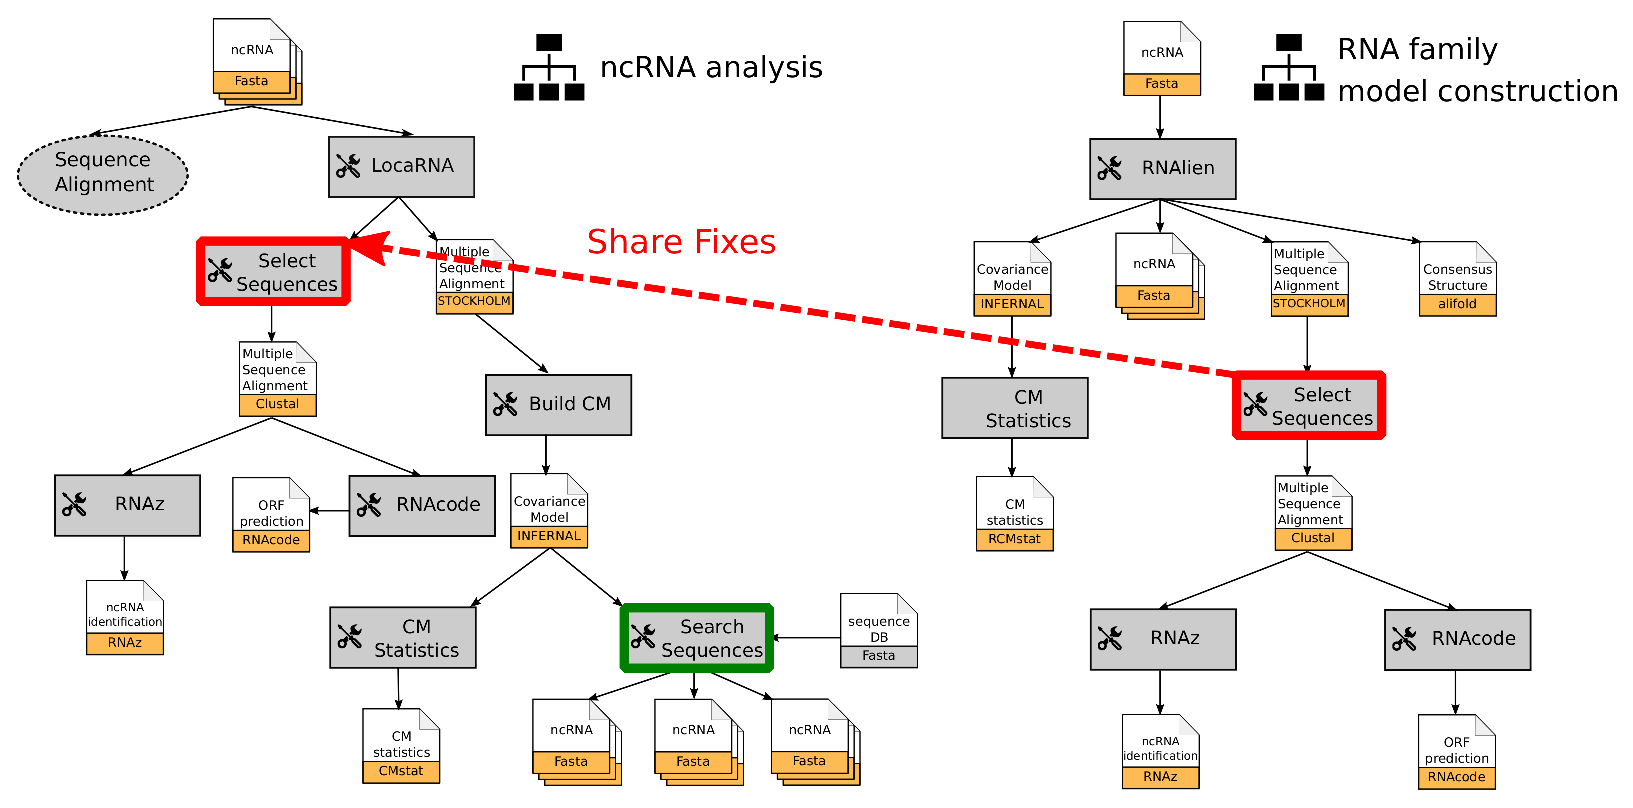
\includegraphics[width=\textwidth]{figures/ncRNAworkflows_simplified_3.eps}
  \end{figure}
}

\frame{
  \frametitle{Collaboration \& Synergistic effects}
   \begin{figure}
     \centering
     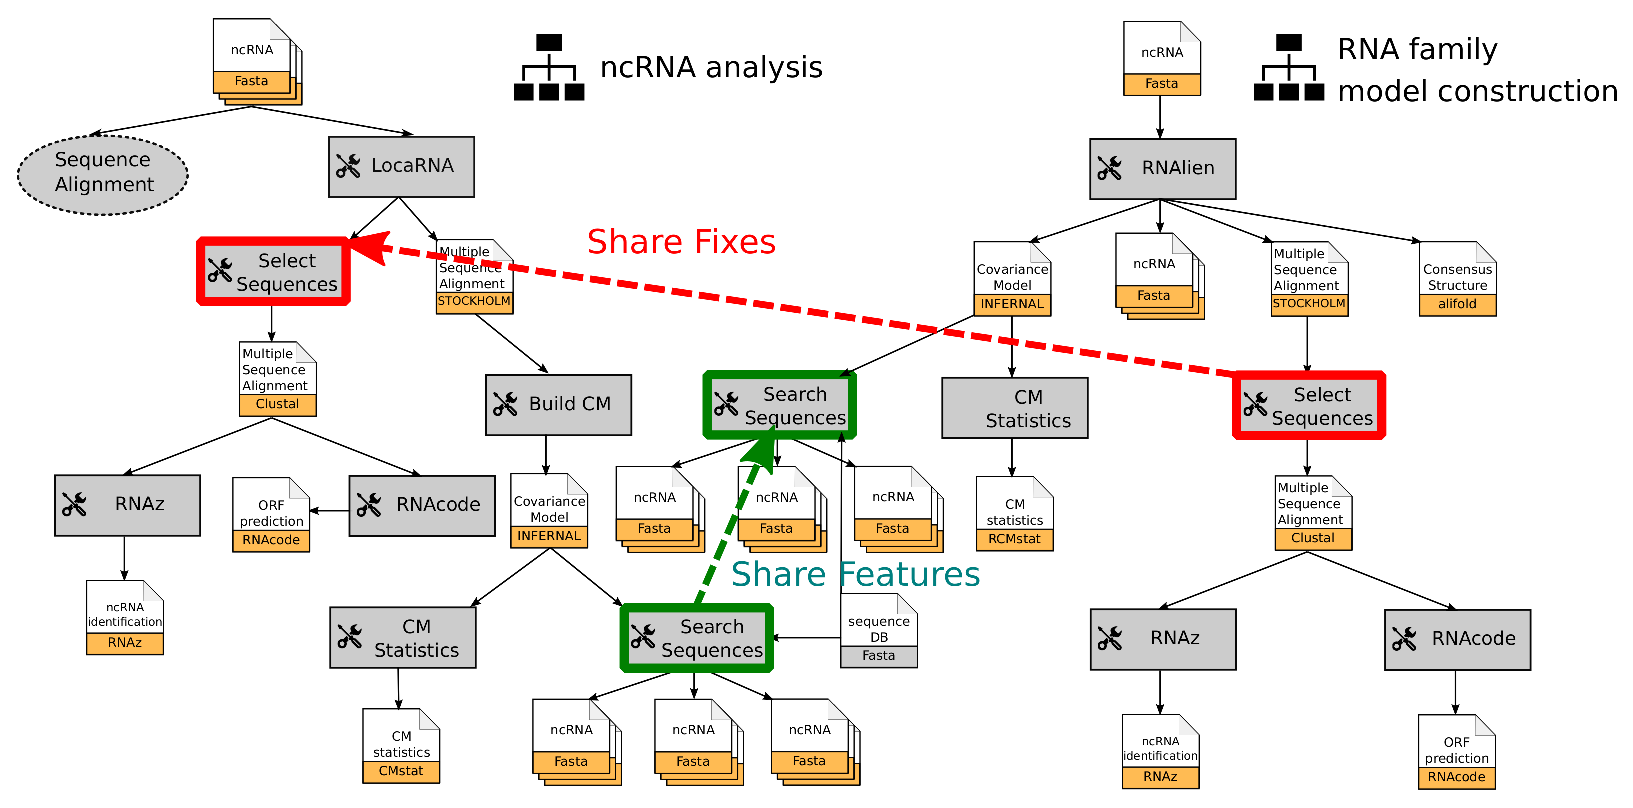
\includegraphics[width=\textwidth]{figures/ncRNAworkflows_simplified_4.eps}
   \end{figure}
}


\frame{
  \frametitle{Community}
  %Personal observation
  Benefits from collaboration and integration\\
  \vspace{0.5cm}
  \onslide<2-> \textbf{12} contributors RNA-workbench
  \onslide<3-> \textbf{54} contributors Galaxy-tools
  \onslide<4-> Open participation, reward, and inclusion
  \vspace{0.5cm}
  \onslide<2->\textbf{Tool authors}
  \begin{itemize}
  \item<5-> Ensure correct application of tool
  \item<6-> Identify missing interfaces between tools
  \item<7-> New ideas for workflows
  \end{itemize}
  \vspace{0.5cm}
  \onslide<8->\textbf{Galaxy developers}
  \begin{itemize}
  \item<9-> Simpler workflow construction
  \item<10-> Authors keep tools updated
  \end{itemize}
   %Benefits from collaboration of multiple tool authors and galaxy developers
   %Authors - bigger audiance for tool
   %Ideas for workflows and best usage of tools
   %Galaxy developers, better interfaces between tools
   %Users more tools and functionality, easier feedback and feature requests? 
 %%  \begin{itemize}
%%   \item Open participation, reward, and inclusion
%%   \item Galaxy, BioConda, BioContainers and BioJS
%%   \item GitHub, IRC, and Gitter
%%   \end{itemize}  
  %%
}


\frame{
  \frametitle{Training \& Usage}
  \onslide<2->\textbf{Training}
  \begin{itemize}
    \item<3-> Training sessions (Introduction, HTS data and \textit{RNA}-seq analyses)
    \item<4-> http://galaxyproject.github.io/training-material
    \item<5-> Galaxy Interactive Tours
  \end{itemize}
  \vspace{0.5cm}
  \onslide<6->\textbf{Using the workbench}
  \begin{itemize}
  \item<7-> docker run -d -p 8080:80 bgruening/galaxy-rna-workbench
  \item<8-> OSX and Windows using the graphical tool Kitematic 
  \end{itemize}  
}

%% \frame{
%%   \frametitle{Training \&Usage}
%%   \begin{itemize}
%%   \item Training sessions (Introduction, HTS data and \textit{RNA}-seq analyses)
%%   \item http://galaxyproject.github.io/training-material
%%   \item Galaxy Interactive Tours
%%   \end{itemize}  
%% }

  %% \frametitle{Implementation \& Usage}
  %% \begin{itemize}
  %% \item<1-> Galaxy framework - reproducibility, usability %Accessiblility - webservice
  %% \item<2-> Docker - deployment, layers (Data, Tours, Documentation) %Workflows, Tools
  %%   %layer figure?
  %% \item<3-> Bioconda - version management, dependencies % staying up-to-date
  %% \item<4-> Continious integration (CI) - testing
  %% \end{itemize}


%% \frame{
%%   \frametitle{Visualisation}
%%   \begin{itemize}
%%   \item General purpose bar chart scatter plot
%%   \item Connection to IGV, UCSC genome browsers
%%   \item Specific \textit{RNA} visualisation Dot plot, dot-bracket, tertiary structure (3D)
%%   \end{itemize}  
%% }


%\frame{
%  \frametitle{Using the workbench}
%  \begin{itemize}
%  \item docker run -d -p 8080:80 bgruening/galaxy-rna-workbench
%  \item OSX and Windows using the graphical tool Kitematic 
%  \end{itemize}  
%}


\frame{
  \frametitle{Acknowledgements \& Thanks}
  \vspace{1cm}
  
\includegraphics[width=1\textwidth]{figures/funding.eps}
}

\frame{
  \frametitle{RNA-seq analysis: trimming, mapping and read count}
  \begin{itemize}
  \item Test for differential gene expression
  \item Quality control - Mapping \& Annotation - Differential expression
  \item Template for customized workflows
  \end{itemize}
  %Workflow Figure
}
\end{document}
